% Provenance (never printed): cycle 4 SVT, "La planete Terre, l'environnement
% et l'action humaine": climate, its past variations and the present change,
% read from data; see sources/book1/PROVENANCE.md. Book 1, grade 9, chapter 1.
% Vocabulary guard: owns climate change (first look; Book 2 g12 re-uses it),
% global warming, temperature anomaly. The greenhouse effect and greenhouse
% gases belong to the chemistry series (grade 8): recalled in prose, never
% defined. Infrared is physics (g10): named in prose only. "Glacial period"
% and "interglacial" belong to Book 2 g12: here "the ice ages and the warmer
% times between them". Physical science only, in the IPCC's calibrated words;
% no policy.
\chapter{مناخ الأرض بين الماضي والحاضر}\label{ch:g9:climate-past-and-present}

لو لم يكن حول الأرض هواء، لكنها عكست الحصة نفسها من ضوء الشمس التي تعكسها
اليوم، لاستقرت درجة حرارة سطحها عند متوسط يقارب \qty{-19}{\degreeCelsius}:
بحار متجمدة، ويابسة متجمدة، في كل مكان. أما متوسطها الحقيقي فنحو
\qty{15}{\degreeCelsius}. والفرق، نحو \qty{34}{\degreeCelsius}، يأتي من بضعة
غازات في الهواء، موجودة بكميات ضئيلة جدًا، تمنع جزءًا من حرارة الأرض من
الإفلات إلى الفضاء. ويتناول هذا الفصل هذه الغازات، \omterm{def:g5:weather-and-climate:climate}{ومناخ} الأرض في الماضي، وكيف
يتغير الآن ولماذا.
% ledger: earth:Tbb, earth:Tsurf (figdata/grade-9/climate_records.py: -19.1 and 14.9 degC, gap 34)

\begin{recall}
\omterm{def:g5:weather-and-climate:climate}{مناخ} مكان ما هو \omterm{def:g1:watching-the-weather:weather}{الطقس} الذي يسود فيه عادة، محسوبًا متوسطه على مدى 30 سنة
(\cref{ch:g5:weather-and-climate}). والطبقة الدنيا من الغلاف الجوي، حيث يحدث
\omterm{def:g1:watching-the-weather:weather}{الطقس}، هي \omterm{def:g8:the-atmosphere:layers}{التروبوسفير} (\cref{ch:g8:the-atmosphere}). وقد جاءت \omterm{def:g8:ice-on-earth:ice-age}{عصور جليدية}
وذهبت، امتدت فيها \omterm{def:g8:ice-on-earth:ice-sheet}{الأغطية الجليدية} بعيدًا عن \omterm{def:g3:continents-and-oceans:poles}{القطبين}؛ وتقلص \omterm{def:g8:ice-on-earth:sea-ice}{الجليد البحري} في
المنطقة القطبية الشمالية منذ 1979 (\cref{ch:g8:ice-on-earth}). وفي الكيمياء
تتعلم أن ثاني أكسيد الكربون والميثان وبخار الماء \emph{غازات دفيئة}: فهي تسمح
لضوء الشمس بالمرور لكنها تمتص الأشعة غير المرئية تحت الحمراء التي تطلقها
الأرض الدافئة، وهذا هو \emph{أثر الدفيئة}؛ وأن حرق الفحم والنفط والغاز يطلق
ثاني أكسيد الكربون.
\end{recall}

\section{أثر الدفيئة ودرجة حرارة الأرض}

يعبر ضوء الشمس الغلاف الجوي ويسخّن الأرض والمحيطات. ومثل كل جسم دافئ، يطلق
السطح الدافئ بدوره طاقة، على شكل أشعة تحت حمراء لا تراها العين. فلو أفلتت كلها
إلى الفضاء، لكانت الأرض ذلك العالم المتجمد الذي في الفقرة الأولى. لكن غازات
الدفيئة في الهواء تمتص كثيرًا من هذه الأشعة تحت الحمراء وتعيد جزءًا منها نحو
الأسفل: فيتلقى السطح طاقة من الشمس ومن الهواء الذي فوقه معًا، ويستقر عند درجة
حرارة أعلى.

\begin{omfigure}
\begin{tikzpicture}[font=\footnotesize, >={Stealth[length=2.4mm]}]
  % ground and atmosphere
  \fill[omLithAlluv] (0,0) rectangle (12,0.5);
  \fill[omSea!45] (0,0.5) rectangle (12,3.4);
  \node[anchor=north east, align=right] at (11.85,3.35) {غلاف جوي فيه\\ غازات الدفيئة};
  \node[anchor=south east] at (11.9,0.05) {الأرض والمحيطات};
  \node[anchor=south west] at (0.15,3.5) {الفضاء};
  % Sun
  \fill[omWxSun] (1.3,5.0) circle (0.45);
  \node at (1.3,4.3) {الشمس};
  % sunlight in
  \draw[->, omWxSun!80!black, line width=2.2pt] (1.7,4.6) -- (2.7,0.55)
    node[pos=0.25, right=2pt, align=left, black] {يدخل ضوء الشمس\\ ويسخّن السطح};
  % infrared out and back
  \draw[->, omWarm, line width=1.6pt, decorate, decoration={snake, amplitude=1mm, segment length=4mm, post length=3mm}]
    (6.0,0.55) -- (6.6,2.6);
  \draw[->, omWarm, line width=1.6pt, decorate, decoration={snake, amplitude=1mm, segment length=4mm, post length=3mm}]
    (6.6,2.7) -- (7.4,5.0) node[right, align=left, black] {جزء يفلت\\ إلى الفضاء};
  \draw[->, omWarm, line width=1.6pt, decorate, decoration={snake, amplitude=1mm, segment length=4mm, post length=3mm}]
    (6.8,2.75) -- (8.6,0.55);
  \node[align=left, anchor=west] at (8.8,1.9) {جزء تمتصه الغازات\\ وتعيده نحو\\ الأسفل};
  \node[align=right, anchor=east] at (5.9,1.3) {السطح الدافئ يطلق\\ أشعة تحت حمراء};
\end{tikzpicture}

{\small أثر الدفيئة، ببساطة (رسم تخطيطي). لولاه لبلغ متوسط حرارة سطح الأرض نحو
\qty{-19}{\degreeCelsius}؛ ومعه يبلغ نحو
\qty{15}{\degreeCelsius}.}
% ledger: earth:Tbb, earth:Tsurf
\label{fig:g9:climate-past-and-present:greenhouse}
\end{omfigure}

أثر الدفيئة طبيعي وضروري: فلولاه لما وُجد ماء سائل على السطح. أما سؤال هذا
الفصل فمختلف: ماذا يحدث لدرجة حرارة الأرض حين تتغير كمية غازات الدفيئة في
الهواء؟

\section{مناخات الماضي}

لقراءة \omterm{def:g5:weather-and-climate:climate}{مناخ} الماضي البعيد، يحفر العلماء في \omterm{def:g8:ice-on-earth:ice-sheet}{الأغطية الجليدية}. ففي كل سنة يسقط
\omterm{def:g4:clouds-rain-snow:precipitation}{الثلج} على القارة القطبية الجنوبية وغرينلاند، ويختلف \omterm{def:g4:clouds-rain-snow:precipitation}{ثلج} الصيف قليلًا عن \omterm{def:g4:clouds-rain-snow:precipitation}{ثلج}
الشتاء. وحين تُدفن الطبقات السنوية وتُضغط فتصير جليدًا، تبقى واحدة فوق الأخرى،
كصفحات كتاب. وكلما كان الجليد أعمق، كان أقدم.
% ledger: eo:ice-core

\begin{omfigure}
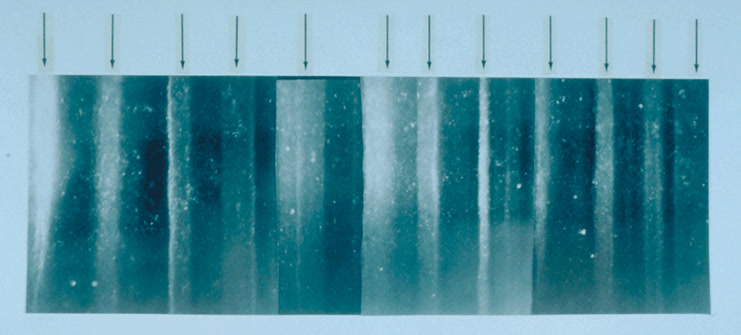
\includegraphics[width=0.78\linewidth]{images/book1/g9-gisp2-layers.jpg}

{\small قطعة من عينة جليدية أسطوانية طولها \qty{19}{cm}، استُخرجت من عمق
\qty{1855}{m} في \omterm{def:g8:ice-on-earth:ice-sheet}{الغطاء الجليدي} لغرينلاند، مضاءة من الأسفل. تشير الأسهم إلى
طبقات الصيف الأفتح، بين طبقات الشتاء الأدكن: إحدى عشرة سنة من \omterm{def:g4:clouds-rain-snow:precipitation}{الثلج}. قسم علم
\omterm{def:g5:weather-and-climate:climate}{المناخ} القديم في الإدارة الوطنية للمحيطات والغلاف الجوي (ملك عام، عبر ويكيميديا
كومنز).}
% ledger: commons:gisp2-layers
\label{fig:g9:climate-past-and-present:ice-core}
\end{omfigure}

تحفظ العينة الجليدية سجلين للماضي. \omterm{def:g4:clouds-rain-snow:precipitation}{فالثلج} نفسه يخبر كم كان الهواء باردًا حين
سقط: فكلما كان الهواء أبرد، صغرت حصة الأشكال الأثقل من الهيدروجين والأكسجين في
\omterm{def:g4:clouds-rain-snow:precipitation}{الثلج}. وحين يُضغط \omterm{def:g4:clouds-rain-snow:precipitation}{الثلج} فيصير جليدًا، تنغلق الفراغات بين حبيباته، فتحبس فقاعات
دقيقة من هواء ذلك الزمن. ويحرر العلماء هذا الهواء القديم في المختبر ويقيسون ما
فيه من ثاني أكسيد الكربون.
% ledger: eo:ice-core

\begin{omfigure}
\begin{tikzpicture}
\begin{axis}[name=temp, omrecord, omage, width=13cm, height=3.9cm, xmin=0, xmax=800,
  xtick={0,100,...,800}, xticklabels={}, ylabel={\foreignlanguage{arabic}{تغير درجة}\\ \foreignlanguage{arabic}{الحرارة \babelsublr{($^\circ$C)}}},
  ylabel style={align=center}, ymin=-11, ymax=5, ytick={-10,-5,0,5}]
  \addplot[omWarm, line width=0.7pt] table[x=age_kyr, y=temp_C] {figdata/out/grade-9-climate_records-edc.dat};
\end{axis}
\begin{axis}[at={(temp.south west)}, anchor=north west, yshift=-0.3cm, omrecord, omage,
  width=13cm, height=3.9cm, xmin=0, xmax=800, xtick={0,100,...,800},
  xlabel={\foreignlanguage{arabic}{آلاف السنين قبل اليوم}}, ylabel={\foreignlanguage{arabic}{ثاني أكسيد}\\ \foreignlanguage{arabic}{الكربون \babelsublr{(ppm)}}},
  ylabel style={align=center}, ymin=160, ymax=320, ytick={180,220,260,300}]
  \addplot[black, line width=0.7pt] table[x=age_kyr, y=co2_ppm] {figdata/out/grade-9-climate_records-icecore.dat};
\end{axis}
\end{tikzpicture}

{\small ثمانمئة ألف سنة مقروءة في جليد القارة القطبية الجنوبية. في الأعلى: تغير
درجة حرارة الهواء في دوم~C، مقارنةً بمتوسط آخر ألف سنة (العينة الجليدية لمشروع
إبيكا في دوم~C، ج.~جوزيل وآخرون، 2007). وفي الأسفل: ثاني أكسيد الكربون في الهواء
المحبوس في الجليد، بالأجزاء في المليون (ب.~بيرايتر وآخرون، 2015). وكلاهما محسوب
متوسطه على خطوات من \num{2000} سنة؛ والزمن يجري من اليسار (الأقدم) إلى اليمين
(اليوم).}
% ledger: data:edc-jouzel, data:co2-bereiter (figdata/grade-9/climate_records.py)
\label{fig:g9:climate-past-and-present:icecore}
\end{omfigure}

يروي المنحنيان القصة نفسها. فمرة بعد مرة، أفسحت أزمنة باردة طويلة، هي \omterm{def:g8:ice-on-earth:ice-age}{العصور
الجليدية}، المجال لأزمنة دافئة أقصر، ثم عادت البرودة. وفي أشد الأوقات برودة، كان
الهواء فوق القارة القطبية الجنوبية أبرد بنحو \qty{9}{\degreeCelsius} مما كان
عليه في آخر ألف سنة؛ وفي أدفأ الأوقات كان أدفأ ببضع درجات. وكان ثاني أكسيد الكربون
يرتفع وينخفض مع درجة الحرارة، بين نحو \qty{175}{ppm} في الأزمنة الباردة ونحو
\qty{300}{ppm} في الأزمنة الدافئة. ونحن نعيش في أحد الأزمنة الدافئة، وقد بدأ حين
انتهى آخر \omterm{def:g8:ice-on-earth:ice-age}{عصر جليدي}.
% ledger: data:edc-jouzel, data:co2-bereiter (figdata/grade-9/climate_records.py: edc min -9.7, max +3.6; CO2 174 to 299 ppm)

\begin{method}[قراءة سجلين جنبًا إلى جنب]
\begin{enumerate}
  \item تحقق من أن السجلين يشتركان في محور الزمن نفسه، وفي أي اتجاه
        يجري الزمن.
  \item اختر تاريخًا على محور الزمن واقرأ كل سجل عند ذلك التاريخ.
  \item ابحث عن القمم والقيعان: هل تأتي في الأوقات نفسها في السجلين
        كليهما؟
  \item قل ما الذي يتحرك معًا، دون أن تقرر بعدُ أي التغيرين سبّب
        الآخر.
\end{enumerate}
\end{method}

\begin{example}[آخر عصر جليدي في العينة الجليدية]
عند \num{20000} سنة قبل اليوم (العدد 20 على محور الزمن)، يكون منحنى درجة
الحرارة عند نحو \qty{-9}{\degreeCelsius} وثاني أكسيد الكربون عند نحو
\qty{190}{ppm}. وفي آخر ألف سنة، يكون منحنى درجة الحرارة قريبًا من 0 وثاني أكسيد
الكربون قريبًا من \qty{280}{ppm}. إذن، في أشد أوقات آخر \omterm{def:g8:ice-on-earth:ice-age}{عصر جليدي} برودة، كان
الهواء فوق القارة القطبية الجنوبية أبرد بنحو \qty{9}{\degreeCelsius}، وكان يحوي
من ثاني أكسيد الكربون أقل بنحو $280 - 190 = \qty{90}{ppm}$، أي أقل بالثلث.
\end{example}
% ledger: data:edc-jouzel, data:co2-bereiter (figdata/grade-9/climate_records.py: 19-21 kyr bins -9.4, 190 ppm; 1 kyr bin 278)

وفي زمن أبعد من ذلك، عرفت الأرض مناخات أدفأ بكثير من أي \omterm{def:g5:weather-and-climate:climate}{مناخ} في آخر
800\,000 سنة. وتقدّر التقييمات العلمية أن آخر مرة بقي فيها سطح الأرض أعلى بمقدار
\qty{2.5}{\degreeCelsius} أو أكثر من مستواه في أواخر القرن التاسع عشر كانت قبل
أكثر من ثلاثة ملايين سنة.
% ledger: ipcc:3myr

\section{سجلات اليوم}

منذ أواخر القرن التاسع عشر، تُقاس درجة الحرارة كل يوم في آلاف \omterm{def:g4:clouds-rain-snow:weather-station}{محطات الأرصاد} على
اليابسة وفي \omterm{def:g2:water-on-earth:ocean}{البحر}، بموازين حرارة محفوظة في الظل. ولمتابعة الكوكب كله، لا يحسب
العلماء متوسط درجات الحرارة نفسها، التي تتوقف على موقع كل محطة، بل متوسط ما
تختلف به كل منها عن قيمتها المعتادة.
% ledger: giss:method

\begin{definition}[شذوذ درجة الحرارة]\label{def:g9:climate-past-and-present:anomaly}
\emph{شذوذ درجة الحرارة}\index{شذوذ درجة الحرارة} هو الفرق بين درجة حرارة
ومتوسطها على مدى فترة مرجعية مختارة. ويكون موجبًا حين يكون الجو أدفأ من ذلك
المتوسط، وسالبًا حين يكون أبرد.
\end{definition}

\begin{omfigure}
\begin{minipage}[c]{0.44\linewidth}\centering
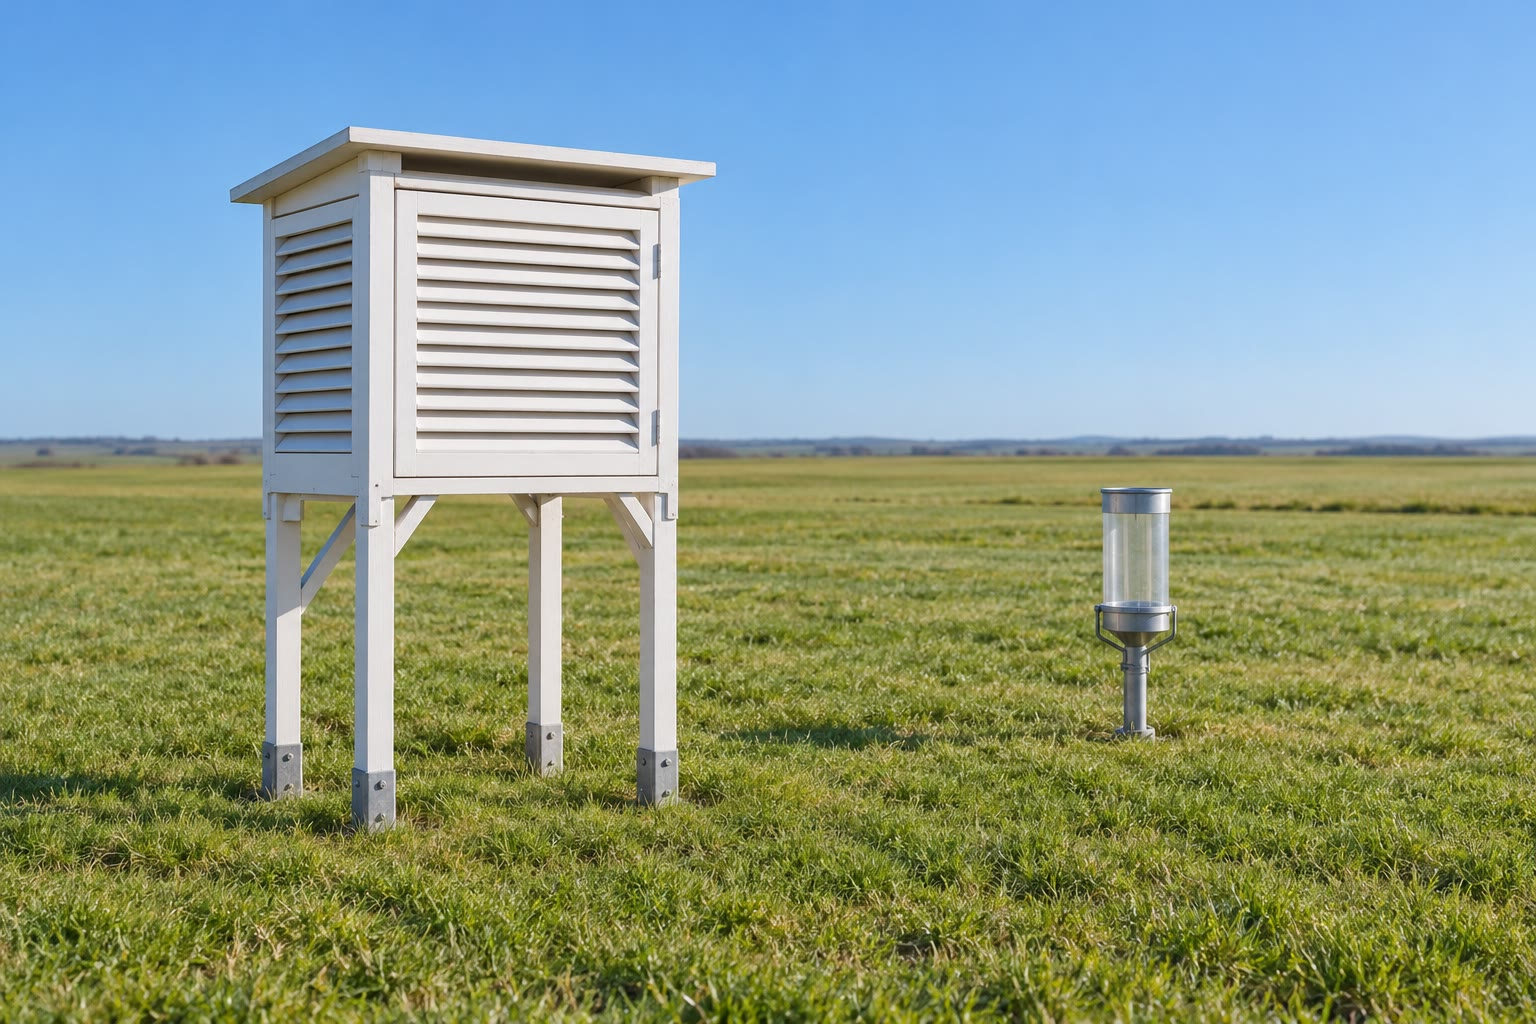
\includegraphics[width=\linewidth]{images/book1/ai/g9-weather-screen.jpg}
\end{minipage}\hfill
\begin{minipage}[c]{0.52\linewidth}\raggedright
{\small \omterm{def:g4:clouds-rain-snow:weather-station}{محطة أرصاد}: الصندوق الأبيض القائم على أرجل، بجوانبه ذات الشرائح، يُبقي
موازين الحرارة في الظل بينما يتدفق الهواء عبره؛ وعلى اليمين مقياس \omterm{def:g4:clouds-rain-snow:precipitation}{مطر} (رسم
توضيحي مولَّد بالذكاء الاصطناعي لمشهد عام).}
\end{minipage}
\label{fig:g9:climate-past-and-present:screen}
\end{omfigure}

فسجل ناسا لدرجة الحرارة العالمية، مثلًا، يعطي شذوذ كل سنة مقارنةً بمتوسط
1951--1980، من محطات اليابسة ومن قياسات سطح \omterm{def:g2:water-on-earth:ocean}{البحر}. وإذا حُسب متوسطه عقدًا بعد
عقد، أظهر ارتفاعًا واضحًا.
% ledger: giss:method, data:gistemp

\begin{omfigure}
\begin{tikzpicture}
\begin{axis}[omrecord, ybar, width=13cm, height=5.6cm, bar width=9pt,
  ymin=-0.45, ymax=1.2, ytick={-0.4,0,0.4,0.8,1.2},
  xtick=data, xticklabels={1880--1889, 1890--1899, 1900--1909, 1910--1919, 1920--1929, 1930--1939, 1940--1949, 1950--1959, 1960--1969, 1970--1979, 1980--1989, 1990--1999, 2000--2009, 2010--2019, 2020--2025},
  x tick label style={rotate=60, anchor=east, font=\scriptsize},
  ylabel={\foreignlanguage{arabic}{شذوذ درجة الحرارة \babelsublr{($^\circ$C)}}}, xmajorgrids=false]
  \addplot[fill=omWarm!70, draw=black!50] table[x expr=\coordindex, y=mean_C]
    {figdata/out/grade-9-climate_records-decades.dat};
\end{axis}
\end{tikzpicture}

{\small درجة حرارة السطح العالمية، عقدًا بعد عقد منذ ثمانينيات القرن التاسع عشر،
على شكل شذوذ مقارنةً بمتوسط 1951--1980؛ ويغطي العمود الأخير السنوات الست
2020--2025. البيانات: سجل GISTEMP لناسا، الإصدار~4.}
% ledger: data:gistemp (figdata/grade-9/climate_records.py)
\label{fig:g9:climate-past-and-present:decades}
\end{omfigure}

\begin{definition}[الاحترار العالمي]\label{def:g9:climate-past-and-present:global-warming}
\emph{الاحترار العالمي}\index{احترار عالمي} هو ارتفاع متوسط درجة حرارة سطح
الأرض، في مجمله، منذ النصف الثاني من القرن التاسع
عشر.
\end{definition}

يصعد السجل ويهبط سنة بعد سنة: فقد تكون سنة أبرد من التي قبلها، لأن \omterm{def:g1:watching-the-weather:weather}{طقس} سنة
كاملة، فوق المحيطات \omterm{def:g3:continents-and-oceans:continent}{والقارات}، يتغير هو أيضًا. لذلك يقارن العلماء، لقياس احترار
ما، متوسطات على مدى سنوات كثيرة، ولا يقارنون أبدًا سنتين
منفردتين.

\begin{omfigure}
\begin{tikzpicture}
\begin{axis}[omrecord, width=13cm, height=5.4cm, xmin=1875, xmax=2030, ymin=-0.6, ymax=1.4,
  xtick={1880,1900,...,2020}, x tick label style={/pgf/number format/1000 sep={}},
  xlabel={\foreignlanguage{arabic}{السنة}}, ylabel={\foreignlanguage{arabic}{شذوذ درجة الحرارة \babelsublr{($^\circ$C)}}},
  legend style={at={(0.2,0.97)}, anchor=north west, draw=none, fill=white, font=\footnotesize}]
  \fill[omWarm!10] (axis cs:1880,-0.6) rectangle (axis cs:1899,1.4);
  \fill[omWarm!10] (axis cs:2015,-0.6) rectangle (axis cs:2024,1.4);
  \addplot[black!70, mark=*, mark size=0.9pt, line width=0.4pt]
    table[x=year, y=anomaly_C] {figdata/out/grade-9-climate_records-annual.dat};
  \addlegendentry{\foreignlanguage{arabic}{كل سنة}}
  \addplot[omWarm, line width=2pt] table[x=year, y=mean_C] {figdata/out/grade-9-climate_records-periods.dat};
  \addlegendentry{\foreignlanguage{arabic}{متوسط فترة}}
  \draw[dashed, black!50] (axis cs:1875,0) -- (axis cs:2030,0);
  \node[font=\scriptsize, fill=white, inner sep=1pt] at (axis cs:1889.5,0.45) {1880--1899};
  \node[font=\scriptsize, fill=white, inner sep=1pt] at (axis cs:2019.5,0.3) {2015--2024};
\end{axis}
\end{tikzpicture}

{\small \omterm{def:g9:climate-past-and-present:anomaly}{شذوذ درجة الحرارة} العالمية في كل سنة من 1880 إلى 2025 (مقارنةً بمتوسط
1951--1980، الخط المتقطع)، مع متوسطي فترتين من مسألة هذا الفصل: 1880--1899
و2015--2024. البيانات: سجل GISTEMP لناسا،
الإصدار~4.}
% ledger: data:gistemp (figdata/grade-9/climate_records.py)
\label{fig:g9:climate-past-and-present:annual}
\end{omfigure}

\begin{method}[قياس الاحترار بين فترتين]
\begin{enumerate}
  \item اختر فترتين لا تقل كل منهما عن عشر سنوات، إحداهما مبكرة والأخرى
        متأخرة، كي تتلاشى تقلبات السنوات المنفردة.
  \item احسب متوسط الشذوذات السنوية لكل فترة.
  \item اطرح المتوسط المبكر من المتأخر: فالنتيجة هي الاحترار بين
        الفترتين، بالدرجات.
  \item اذكر السجل والفترتين اللتين استعملتها: فسجل آخر، أو فترات
        أخرى، تعطي عددًا مختلفًا قليلًا.
\end{enumerate}
\end{method}

\begin{example}[الاحترار منذ سبعينيات القرن العشرين]
في سجل ناسا، متوسط شذوذات السنوات العشر 1970--1979 هو
\qty{0.03}{\degreeCelsius}، ومتوسط شذوذات 2010--2019 هو
\qty{0.80}{\degreeCelsius}. فالاحترار بين هذين العقدين هو
$0.80 - 0.03 = \qty{0.77}{\degreeCelsius}$، في أربعين سنة: أي نحو
\qty{0.19}{\degreeCelsius} لكل عقد. أما السنوات المنفردة، التي يفصل بينها أربعون
سنة أيضًا، فتعطي أجوبة مختلفة جدًا: فعام 1976 ($-0.10$) مقابل عام 2016
(1.01) يعطي \qty{1.11}{\degreeCelsius}، لكن عام 1979 (0.16) مقابل عام 2011
(0.61) لا يعطي إلا \qty{0.45}{\degreeCelsius}.
\end{example}
% ledger: data:gistemp (figdata/grade-9/climate_records.py: decade_1970s 0.03, decade_2010s 0.80; annual 1976 -0.10, 2016 1.01, 1979 0.16, 2011 0.61)

يُقاس ثاني أكسيد الكربون في الهواء مباشرة منذ مارس 1958، في مرصد يقع على \omterm{def:g4:world-physical-map:altitude}{ارتفاع}
نحو \qty{3400}{m} على سفوح \omterm{def:g4:volcanoes-earthquakes-first-look:volcano}{بركان} ماونا لوا، في هاواي. وفي عام 1959 كان متوسطه
السنوي \qty{316}{ppm}؛ وبحلول عام 2025 بلغ \qty{427}{ppm}، أي أعلى بكثير من
\qty{300}{ppm} التي لم يتجاوزها قط في 800\,000 سنة من الجليد. وهو يرتفع أسرع
فأسرع: بأقل من \qty{1}{ppm} في السنة في ستينيات القرن العشرين، وبأكثر من
\qty{2.5}{ppm} في السنة في السنوات العشر الأخيرة.
% ledger: gml:keeling, data:co2-mlo, data:co2-bereiter (figdata/grade-9/climate_records.py: 315.98, 427.35, 0.86 and 2.63 ppm/yr; ice core max 298.6)

\begin{omfigure}
\begin{tikzpicture}
\begin{axis}[omrecord, width=12cm, height=5cm, xmin=1955, xmax=2030,
  ymin=290, ymax=440, ytick={300,350,400}, xtick={1960,1970,...,2020},
  x tick label style={/pgf/number format/1000 sep={}},
  xlabel={\foreignlanguage{arabic}{السنة}}, ylabel={\foreignlanguage{arabic}{ثاني أكسيد الكربون \babelsublr{(ppm)}}}]
  \addplot[black, line width=0.9pt, mark=*, mark size=0.8pt] table[x=year, y=co2_ppm] {figdata/out/grade-9-climate_records-co2.dat};
  \draw[dashed, omWarm] (axis cs:1955,300) -- (axis cs:2030,300);
\end{axis}
\end{tikzpicture}

{\small ثاني أكسيد الكربون في الهواء في ماونا لوا، هاواي، متوسطات سنوية
1959--2025 (مختبر الرصد العالمي التابع للإدارة الوطنية للمحيطات والغلاف الجوي،
ومعهد سكريبس لعلوم المحيطات). والخط المتقطع عند \qty{300}{ppm} يقارب أعلى مستوى
وُجد في 800\,000 سنة من جليد القارة القطبية الجنوبية.}
% ledger: data:co2-mlo, data:co2-bereiter (figdata/grade-9/climate_records.py)
\label{fig:g9:climate-past-and-present:co2}
\end{omfigure}

\begin{dated}{2025}
بلغ المتوسط السنوي لثاني أكسيد الكربون في ماونا لوا \qty{427.35}{ppm} عام
2025. وفي سجل ناسا، كانت أدفأ سنة منذ 1880 هي 2024، بشذوذ بلغ
\qty{1.28}{\degreeCelsius} مقارنةً بمتوسط 1951--1980.
% ledger: data:co2-mlo, data:gistemp (figdata/grade-9/climate_records.py)
\end{dated}

\omterm{def:g2:water-on-earth:ocean}{والبحر} يرتفع أيضًا. فمنذ 1993، تقيس الأقمار الصناعية ارتفاع سطح \omterm{def:g2:water-on-earth:ocean}{البحر} في أنحاء
الكرة الأرضية كلها: ويرتفع خط اتجاه سجلها بنحو \qty{3.2}{mm} في السنة، أي نحو
\qty{10}{cm} في ثلاثين سنة. وأمران يرفعان \omterm{def:g2:water-on-earth:ocean}{البحر}: الماء الذي يسخن يتمدد، والجليد
الذائب على اليابسة يضيف ماءً إلى \omterm{def:g2:water-on-earth:ocean}{المحيط}. والجليد يتقلص: \omterm{def:g8:ice-on-earth:glacier}{فالأنهار الجليدية}
الجبلية تتراجع في كل مكان تقريبًا، وفقد جليد الصيف البحري في المنطقة القطبية
الشمالية قرابة نصف امتداده منذ 1979 (\cref{ch:g8:ice-on-earth}).
% ledger: data:gmsl-lsa (figdata/grade-9/climate_records.py: 3.18 mm/yr; 101 mm 1993-2024), ipcc:b1-ice, nsidc:ice-shelves, data:b1-nsidc-sea-ice

\begin{omfigure}
\begin{tikzpicture}
\begin{axis}[omrecord, width=12cm, height=4.8cm, xmin=1992, xmax=2026,
  ymin=-30, ymax=100, xtick={1995,2000,...,2025},
  x tick label style={/pgf/number format/1000 sep={}},
  xlabel={\foreignlanguage{arabic}{السنة}}, ylabel={\foreignlanguage{arabic}{مستوى البحر \babelsublr{(mm)}}},
  legend style={at={(0.02,0.97)}, anchor=north west, draw=none, fill=white, font=\footnotesize}]
  \addplot[omCold, mark=*, mark size=1.1pt, line width=0.6pt] table[x=year, y=gmsl_mm] {figdata/out/grade-9-climate_records-sea.dat};
  \addlegendentry{\foreignlanguage{arabic}{المتوسط السنوي}}
  \addplot[omWarm, dashed, line width=0.9pt] table[x=year, y=gmsl_mm] {figdata/out/grade-9-climate_records-sea-trend.dat};
  \addlegendentry{\foreignlanguage{arabic}{خط الاتجاه}}
\end{axis}
\end{tikzpicture}

{\small متوسط \omterm{def:g4:world-physical-map:altitude}{مستوى سطح البحر} العالمي كما تقيسه الأقمار الصناعية، متوسطات سنوية
1993--2024، مقارنةً بمستوى مرجعي، وخط اتجاهه (مختبر قياس الارتفاع بالأقمار
الصناعية التابع للإدارة الوطنية للمحيطات والغلاف الجوي).}
% ledger: data:gmsl-lsa (figdata/grade-9/climate_records.py)
\label{fig:g9:climate-past-and-present:sea}
\end{omfigure}

\section{تغير المناخ وأسبابه}

\begin{definition}[تغير المناخ]\label{def:g9:climate-past-and-present:climate-change}
\emph{تغير المناخ}\index{تغير المناخ} تغيّر في \omterm{def:g5:weather-and-climate:climate}{مناخ} الأرض، أو \omterm{def:g5:weather-and-climate:climate}{مناخ} منطقة ما،
يدوم عقودًا أو أكثر: تغيّر في متوسط درجة حرارته، أو أمطاره، أو رياحه، أو جليده،
لا مجرد فصل واحد غير عادي.
\end{definition}

لقد \omterm{def:g9:climate-past-and-present:climate-change}{تغير المناخ} دائمًا، كما تبين العينات الجليدية. أما الجديد فهو سرعة التغير
الحالي، وسببه. فعلماء من أنحاء العالم كله يقيّمون بانتظام ما نُشر عن \omterm{def:g5:weather-and-climate:climate}{المناخ}، في
تقارير الهيئة الحكومية الدولية المعنية \omterm{def:g9:climate-past-and-present:climate-change}{بتغير المناخ}. وتزن هذه التقارير مدى
اليقين في كل عبارة، بكلمات مختارة بعناية.

وفي هذه التقارير، لكل كلمة من الكلمات أدناه معنى ثابت: عدد الفرص من 100 لأن
تكون العبارة صحيحة.

\begin{center}
{\small
\begin{tabular}{|l|c||l|c|}
\hline
\emph{مؤكد تقريبًا} & من 99 إلى 100 & \emph{مرجح} & من 66 إلى 100 \\
\emph{مرجح للغاية} & من 95 إلى 100 & \emph{متساوي الاحتمال تقريبًا} & من 33 إلى 66 \\
\emph{مرجح جدًا} & من 90 إلى 100 & \emph{غير مرجح} & من 0 إلى 33 \\
\hline
\end{tabular}}
\end{center}
% ledger: ipcc:likelihood

\noindent وقليل من العبارات لا يحمل أيًّا من هذه الكلمات: فهي تُقدَّم بوصفها
حقائق، مثل «إنه أمر \emph{لا لبس فيه}». وحين تقرأ خبرًا صحفيًا عن \omterm{def:g5:weather-and-climate:climate}{المناخ}، ابحث
عن هذه الكلمات، ولاحظ أيها يحتفظ به الخبر وأيها
يسقطه.
% ledger: ipcc:unequivocal

ويقرر التقييم المنشور عام 2021 ما يلي.
\begin{itemize}
  \item مما \emph{لا لبس فيه} أن التأثير البشري قد سخّن الغلاف الجوي
        \omterm{def:g2:water-on-earth:ocean}{والمحيط} واليابسة.
  \item كانت درجة حرارة السطح العالمية في 2011--2020 أعلى بنحو
        \qty{1.1}{\degreeCelsius} مما كانت عليه في 1850--1900، وكان كل عقد
        من العقود الأربعة الأخيرة أدفأ من أي عقد سبقه منذ
        1850.
  \item الاحترار الناجم عن الإنسان من 1850--1900 إلى 2010--2019 يتراوح،
        على نحو \emph{مرجح}، بين 0.8 و\qty{1.3}{\degreeCelsius}، وأفضل
        تقدير له \qty{1.07}{\degreeCelsius}: أي نحو الاحترار المرصود كله.
        أما الأسباب الطبيعية مجتمعة فلم تغير درجة الحرارة إلا بمقدار
        يتراوح بين $-0.1$ و$+\qty{0.1}{\degreeCelsius}$.
  \item كان ثاني أكسيد الكربون في الهواء عام 2019 أعلى منه في أي وقت
        خلال مليوني سنة على الأقل (\emph{بثقة عالية})؛ وقد ارتفع بنسبة
        47~\% منذ 1750.
  \item التأثير البشري هو \emph{على نحو مرجح جدًا} السبب الرئيسي لتراجع
        \omterm{def:g8:ice-on-earth:glacier}{الأنهار الجليدية} منذ تسعينيات القرن العشرين ولتقلص \omterm{def:g8:ice-on-earth:sea-ice}{الجليد البحري} في
        المنطقة القطبية الشمالية؛ وهو \emph{على نحو مرجح جدًا} السبب الرئيسي
        لارتفاع البحر منذ 1971 على الأقل.
\end{itemize}
% ledger: ipcc:unequivocal, ipcc:gsat-2011-2020, ipcc:decades, ipcc:attribution, ipcc:co2-2myr, ipcc:b1-ice, ipcc:sea-level-obs

\begin{history}[منحنى تشارلز ديفيد كيلينغ]
في مارس 1958، بدأ كيميائي شاب في معهد سكريبس لعلوم المحيطات، هو تشارلز ديفيد
كيلينغ، يقيس ثاني أكسيد الكربون في الهواء على ماونا لوا، عاليًا فوق \omterm{def:g2:water-on-earth:ocean}{البحر}
وبعيدًا عن أي مدينة. وقد استمرت قياساته منذ ذلك الحين: فهي أطول سجل لثاني أكسيد
الكربون مقيس مباشرة في الهواء، والمنحنى الذي ترسمه، صاعدًا سنة بعد سنة، يحمل
اسمه: \emph{منحنى كيلينغ}.
% ledger: gml:keeling
\end{history}

لماذا يتبع الاحترار ثاني أكسيد الكربون؟ حرق الفحم والنفط والغاز يطلق ثاني أكسيد
الكربون؛ ومزيد من ثاني أكسيد الكربون في الهواء يعني أن جزءًا أكبر من الأشعة تحت
الحمراء التي يطلقها السطح يُمتص ويُعاد نحو الأسفل، فيسخن السطح. ويضيف بخار
الماء والميثان وغازات الدفيئة الأخرى إلى هذا الأثر. والماضي والحاضر متفقان:
ففي العينات الجليدية كما في سجلات اليوم، ترتفع درجة حرارة الأرض وثاني أكسيد
الكربون فيها وتنخفضان معًا.
% ledger: ipcc:attribution, ipcc:co2-2myr

\section{تمارين}

\begin{exercise}[$\star$]\label{exo:g9:climate-past-and-present:1}
% ledger: earth:Tbb, earth:Tsurf
(أ) ما متوسط درجة حرارة سطح الأرض لولا أثر الدفيئة؟ (ب) وما هو بوجوده؟
(ج) بكم درجة يسخّن أثر الدفيئة السطح؟ (د) سمِّ غازين من غازات
الدفيئة.
\end{exercise}

\begin{exercise}[$\star$]\label{exo:g9:climate-past-and-present:2}
\omterm{def:g1:watching-the-weather:weather}{طقس} أم \omterm{def:g5:weather-and-climate:climate}{مناخ}؟ (أ) أمطرت طوال يوم أمس. (ب) الصيف في هذه المنطقة حار جاف.
(ج) كانت سنوات 2010--2019 أدفأ من سنوات 1980--1989 في العالم كله. (د) سيكون
الأسبوع القادم باردًا.
\end{exercise}

\begin{exercise}[$\star$]\label{exo:g9:climate-past-and-present:3}
% ledger: commons:gisp2-layers
انظر إلى صورة قطعة العينة الجليدية. (أ) ما طول القطعة، وكم سنة من \omterm{def:g4:clouds-rain-snow:precipitation}{الثلج} تحوي؟
(ب) جد متوسط سُمك طبقة سنة واحدة، بالسنتيمترات. (ج) لماذا يكون أعمق جليد في
\omterm{def:g8:ice-on-earth:ice-sheet}{الغطاء الجليدي} هو الأقدم؟
\end{exercise}

\begin{exercise}[$\star$]\label{exo:g9:climate-past-and-present:4}
متوسط درجة حرارة شهر يوليو في بلدة على مدى 1991--2020 هو
\qty{21.0}{\degreeCelsius}. أعطِ \omterm{def:g9:climate-past-and-present:anomaly}{شذوذ درجة الحرارة} لشهر يوليو متوسطه
(أ) \qty{22.4}{\degreeCelsius}؛ (ب) \qty{20.3}{\degreeCelsius}؛
(ج) \qty{21.0}{\degreeCelsius}. (د) ماذا يعني الشذوذ السالب؟
\end{exercise}

\begin{exercise}[$\star\star$]\label{exo:g9:climate-past-and-present:5}
% ledger: data:gistemp (figdata/grade-9/climate_records.py)
استعمل مخطط الأعمدة للعقود. (أ) أي العقود كانت أبرد من متوسط 1951--1980؟
(ب) اقرأ شذوذ عقد 1980--1989 وعقد 2010--2019. (ج) بكم ازداد الشذوذ بين هذين
العقدين؟ (د) هل الارتفاع منتظم من عقد إلى الذي يليه على مدى السجل
كله؟
\end{exercise}

\begin{exercise}[$\star\star$]\label{exo:g9:climate-past-and-present:6}
% ledger: data:co2-mlo (figdata/grade-9/climate_records.py)
في ماونا لوا، كان المتوسط السنوي لثاني أكسيد الكربون \qty{315.98}{ppm} عام
1959، و\qty{324.62}{ppm} عام 1969، و\qty{401.01}{ppm} عام 2015، و\qty{427.35}{ppm} عام 2025. (أ) ما
متوسط الارتفاع في السنة من 1959 إلى 1969؟ (ب) ومن 2015 إلى 2025؟ (ج) كم مرة
كان الارتفاع أسرع في الفترة الثانية؟ (د) بكم في المئة ازداد ثاني أكسيد الكربون
من 1959 إلى 2025؟
\end{exercise}

\begin{exercise}[$\star\star$]\label{exo:g9:climate-past-and-present:7}
% ledger: data:edc-jouzel, data:co2-bereiter
استعمل سجل الثمانمئة ألف سنة. (أ) اكتب 800\,000 سنة بالترميز العلمي. (ب) منذ
كم من الزمن تقريبًا كانت آخر مرة بلغ فيها الدفء مثل اليوم، قبل زمننا الدافئ؟
(ج) ما مستوى ثاني أكسيد الكربون الذي كان في الهواء حينئذ؟ (د) هل ترتفع درجة
الحرارة وثاني أكسيد الكربون وينخفضان في الأوقات
نفسها؟
\end{exercise}

\begin{exercise}[$\star\star$]\label{exo:g9:climate-past-and-present:8}
% ledger: data:gmsl-lsa (figdata/grade-9/climate_records.py)
يرتفع \omterm{def:g2:water-on-earth:ocean}{البحر} بنحو \qty{3.2}{mm} في السنة. (أ) كم يكون ذلك في 10 سنوات،
بالسنتيمترات؟ (ب) لو حافظ على هذا المعدل، فكم سيرتفع بين 2025 و2100؟ (ج) اذكر
سببين لارتفاع البحر. (د) هل يرفع ذوبان \omterm{def:g8:ice-on-earth:sea-ice}{الجليد البحري} في المنطقة القطبية
الشمالية \omterm{def:g2:water-on-earth:ocean}{البحر}؟ علّل.
\end{exercise}

\begin{exercise}[$\star\star$]\label{exo:g9:climate-past-and-present:9}
% ledger: ipcc:likelihood
بكلمات الهيئة الحكومية الدولية، كم فرصة من 100، على الأقل، لكل عبارة أن تكون
صحيحة؟ (أ) «من \emph{المرجح جدًا}\ldots» (ب) «من \emph{المرجح}\ldots» (ج) «من
\emph{المؤكد تقريبًا}\ldots» (د) تكتب صحيفة «العلماء متأكدون من أن» عن عبارة
يصفها التقرير بأنها \emph{مرجحة}. ما الخطأ؟
\end{exercise}

\begin{exercise}[$\star\star$]\label{exo:g9:climate-past-and-present:10}
يقول صديق: «كان هذا الشتاء الأبرد منذ عشر سنوات حيث أعيش، إذن فالأرض لا تزداد
احترارًا.» اشرح، مستعملًا الكلمات \emph{\omterm{def:g1:watching-the-weather:weather}{طقس}} و\emph{\omterm{def:g5:weather-and-climate:climate}{مناخ}} و\emph{عالمي}، لماذا
لا تصمد هذه الحجة.
\end{exercise}

\begin{exercise}[$\star\star\star$]\label{exo:g9:climate-past-and-present:11}
% ledger: data:co2-bereiter, data:co2-mlo, ipcc:co2-2myr, ipcc:erf-2xco2
في أشد أوقات آخر \omterm{def:g8:ice-on-earth:ice-age}{عصر جليدي} برودة، قبل نحو $2 \times 10^4$ سنة، كان الهواء يحوي
نحو \qty{190}{ppm} من ثاني أكسيد الكربون؛ وقبيل العصر الصناعي، نحو
\qty{280}{ppm}؛ وفي 2025، نحو \qty{427}{ppm}. (أ) بكم ارتفع ثاني أكسيد الكربون
من \omterm{def:g8:ice-on-earth:ice-age}{العصر الجليدي} إلى العصر الصناعي، وفي كم سنة؟ (ب) بكم ارتفع من العصر الصناعي
إلى 2025؟ اعتبر 1750 بداية العصر الصناعي. (ج) قارن الارتفاعين: في المقدار، وفي
متوسط المعدل السنوي، مستعملًا الترميز العلمي. (د) ماذا تقول الهيئة الحكومية
الدولية عن مستوى ثاني أكسيد الكربون اليوم مقارنةً بالماضي؟
\end{exercise}

\begin{exercise}[$\star\star\star$]\label{exo:g9:climate-past-and-present:12}
% ledger: ipcc:attribution, ipcc:observed-2010-2019
يعطي تقييم الهيئة الحكومية الدولية الاحترار المرصود من 1850--1900 إلى
2010--2019 بنحو \qty{1.06}{\degreeCelsius}، والاحترار الناجم عن الإنسان بأنه
يتراوح، على نحو \emph{مرجح}، بين 0.8 و\qty{1.3}{\degreeCelsius} (وأفضل تقدير
\qty{1.07}{\degreeCelsius})؛ أما الأسباب الطبيعية مجتمعة فيُعطى أثرها بين
$-0.1$ و$+\qty{0.1}{\degreeCelsius}$. (أ) قارن أفضل تقدير للاحترار الناجم عن
الإنسان بالاحترار المرصود. (ب) هل يمكن للأسباب الطبيعية وحدها أن تفسر الاحترار
المرصود؟ علّل. (ج) ماذا تعني \emph{مرجح} في هذه الجملة؟
\end{exercise}

\section{مسألة: ميزان حرارة الكوكب}

\begin{problem}[{مسألة نهاية الأسبوع --- يُحسب احترار الأرض من سجل ناسا لدرجة
الحرارة، ثم يوضع جنبًا إلى جنب مع ثاني أكسيد الكربون
والبحر}]
\label{pb:g9:climate-past-and-present:1}
% ledger: data:gistemp, data:co2-mlo, data:gmsl-lsa, ipcc:gsat-2011-2020 (figdata/grade-9/climate_records.py)
يعطي الجدول \omterm{def:g9:climate-past-and-present:anomaly}{شذوذ درجة الحرارة} العالمية في سجل ناسا (مقارنةً بمتوسط 1951--1980)
لبعض مجموعات السنوات، وسجلات أخرى من الفصل.

\begin{center}
{\small
\begin{tabular}{|l|c|}
\hline
متوسط الشذوذ، 1880--1899 & \qty{-0.22}{\degreeCelsius} \\
متوسط الشذوذ، 1951--1980 & \qty{0.00}{\degreeCelsius} \\
متوسط الشذوذ، 2015--2024 & \qty{0.98}{\degreeCelsius} \\
ثاني أكسيد الكربون في ماونا لوا، 1959 / 2025 & \qty{316}{ppm} / \qty{427}{ppm} \\
خط اتجاه مستوى \omterm{def:g2:water-on-earth:ocean}{البحر} من الأقمار الصناعية، منذ 1993 & \mbox{\textdir TLT\qty{3.2}{mm}} في السنة \\
\hline
\end{tabular}}
\end{center}

\noindent\textbf{الجزء الأول --- العقود.}\par\nopagebreak
\begin{enumerate}[beginpenalty=10000]
  \item لماذا يساوي شذوذ الفترة 1951--1980 صفرًا تمامًا؟
  \item هل كانت الفترة 1880--1899 أدفأ أم أبرد من 1951--1980؟ وبكم؟
  \item هل كانت الفترة 2015--2024 أدفأ أم أبرد من 1951--1980؟ وبكم؟
  \item احسب احترار الفترة 2015--2024 مقارنةً بالفترة 1880--1899.
\end{enumerate}

\noindent\textbf{الجزء الثاني --- ثاني أكسيد الكربون.}\par\nopagebreak
\begin{enumerate}[resume, beginpenalty=10000]
  \item بكم جزءًا في المليون ارتفع ثاني أكسيد الكربون بين 1959 و2025؟
  \item بأي نسبة مئوية من قيمته عام 1959؟
  \item في العينات الجليدية، لم يتجاوز ثاني أكسيد الكربون قط نحو
        \qty{300}{ppm} في 800\,000 سنة. فبكم تتجاوزها قيمة عام
        2025؟
  \item اشرح في جملتين كيف يسخّن مزيد من ثاني أكسيد الكربون في الهواء
        السطح.
\end{enumerate}

\noindent\textbf{الجزء الثالث --- البحر.}\par\nopagebreak
\begin{enumerate}[resume, beginpenalty=10000]
  \item كم ارتفع \omterm{def:g2:water-on-earth:ocean}{البحر} من 1993 إلى 2025 بمعدل الجدول، بالسنتيمترات؟
  \item اذكر سببي هذا الارتفاع.
  \item تعطي الهيئة الحكومية الدولية احترار 2011--2020 مقارنةً بالفترة
        1850--1900 بنحو \qty{1.09}{\degreeCelsius}. فهل جوابك عن
        السؤال~4 من الحجم نفسه؟ اذكر سببًا واحدًا لاختلاف العددين
        قليلًا.
  \item اكتب الجملة التي يمكن لصحفي علمي أن ينشرها: «منذ نهاية القرن
        التاسع عشر، ارتفعت حرارة سطح الأرض بنحو
        \ldots»
\end{enumerate}
\end{problem}
